\section{KULLANILAN TEKNOLOJİLER}
Bu çalışmada kullanılan teknolojilerin tercih sebepleri ve özellikleri detaylıca aşağıda bahsedilmiştir.
\subsection{Docker}\label{subsec:docker}
Docker, yazılım uygulamalarını konteynerlere paketleme ve dağıtma konusunda kullanılan bir platformdur. Bu teknoloji, uygulamaların bağımsız bir şekilde çalışabilmesini sağlar ve kurulum ve dağıtım süreçlerini kolaylaştırır. Docker, bir uygulamanın çalışması için gerekli olan tüm bağımlılıkları içeren bir konteyner oluşturmanızı sağlar. Bu konteyner, farklı ortamlarda (geliştirme, test, üretim) aynı şekilde çalışabilir, uyumluluk sorunlarını en aza indirir ve uygulamaların taşınabilirliğini artırır. Docker, yüksek verimlilik ve izolasyon sağlar, kaynakların daha etkili kullanılmasını sağlar ve sistem yönetimini kolaylaştırır \cite{docker}.\\
Bu çalışmada kullanılan Docker özellikleri:
\begin{itemize}
  \item \textbf{Docker compose}: Docker ortamında birden fazla konteyneri yönetmek için kullanılan bir araçtır. Docker Compose, bir YAML dosyası aracılığıyla konteynerleri tanımlamanıza ve yapılandırmanıza olanak sağlar. Bu YAML dosyasında, farklı konteynerlerin konfigürasyonları, ağ bağlantıları, bağımlılıkları ve diğer özellikleri belirtilebilir. Docker Compose, bu dosyayı okuyarak ve yorumlayarak belirtilen konteynerleri oluşturur, başlatır ve durdurur. Böylece birden fazla konteynerin aynı ortamda birlikte çalışmasını kolaylaştırır.
  \item \textbf{Docker Engine API}: Docker ortamını yönetmek için kullanılan bir programlama arabirimidir. Docker Engine, Docker'ın temel bileşenidir ve konteynerlerin oluşturulması, çalıştırılması ve yönetilmesi gibi işlemleri gerçekleştirir. Docker Engine API, Docker ortamının komut satırı arayüzünün (CLI) ötesine geçerek programatik olarak Docker ortamını kontrol etmenizi sağlar. Bu API, Docker ile etkileşim kurmanızı ve Docker işlemlerini otomatikleştirmenizi sağlayan bir dizi yöntem ve işlev sağlar. Docker Engine API, HTTP üzerinden erişilebilen bir RESTful API olarak sunulur ve Docker komutlarını programlamaya entegre etmenize olanak tanır \cite{docker_api_reference}.
\end{itemize}

\subsection{Laravel}
Laravel, PHP tabanlı bir web uygulama geliştirme framework'üdür. MVC (Model-View-Controller) tasarım desenini benimser ve geliştiricilere web uygulamaları oluşturmak için bir dizi kullanışlı özellik sunar. Laravel, güçlü bir yönlendirme sistemi, otomatik olarak oluşturulan SQL sorguları, oturum yönetimi, veritabanı migrasyonları, önbellekleme, form doğrulama gibi birçok bileşeni içerir. Bu bileşenler, geliştirme sürecini hızlandırır ve kod tekrarını azaltır. Laravel'in geniş bir topluluğu vardır ve bu da destek almak ve kaynaklara erişmek açısından avantaj sağlar \cite{laravel_documentation}.\\
Bu çalışmada kullanılan Laravel özelliklerine kısaca bir göz atalım:
\begin{itemize}
  \item \textbf{Migration (migrasyon)} : Laravel, veritabanı tablolarını oluşturmak ve yönetmek için migrasyonları kullanır. Migrasyonlar, veritabanı şemalarını kod olarak temsil eder ve veritabanı yapısının kolayca değiştirilmesini ve sürdürülmesini sağlar.
  \item \textbf{Model} : Laravel'de model, veritabanı tablolarıyla ilişkilendirilen veri erişim katmanını temsil eder. Model sınıfları, veritabanı işlemlerini gerçekleştirmek ve verileri işlemek için kullanılır.
  \item \textbf{Request} :  Laravel, HTTP isteklerini işlemek için request (istek) sınıflarını kullanır. Bu sınıflar, gelen istek verilerini doğrulamak, işlemek ve manipüle etmek için kullanılır.
  \item \textbf{Controller} : Laravel'de controller (denetleyici), HTTP isteklerini yöneten ve ilgili iş mantığını uygulayan sınıflardır. Bir controller, bir veya daha fazla işlem (action) içerir ve bu işlemler, isteklere yanıt olarak çalıştırılır.
  \item \textbf{Route} : Laravel, yönlendirme (routing) mekanizmasıyla istekleri doğru controller ve işlemle eşleştirir. Route dosyalarında, URL'leri belirleyebilir, istek yönlendirmelerini tanımlayabilir ve parametreleri yakalayabilirsiniz.
  \item \textbf{Queue} : Laravel, işleri (jobs) arkaplanda sıralı olarak çalıştırmak için kuyruk (queue) sistemini destekler. Kuyruklar, yoğun işlem yükü altında olan uygulamalarda işleri geciktirir ve daha sonra işlerin işlenmesini sağlar.
  \item \textbf{Auth} : Laravel'in sağladığı kimlik doğrulama (authentication) sistemi. Auth bileşeni, kullanıcı kaydı, oturum yönetimi, şifre sıfırlama gibi kullanıcı kimlik doğrulama işlemlerini kolaylaştırır.
  \item \textbf{Event/Listener} : Laravel'de "Event" ve "Listener" kavramları, olay tabanlı programlama yaklaşımını desteklemek için kullanılır. Bir "Event" (olay), uygulamanızda gerçekleşen belirli bir eylemi veya durumu temsil eder.
  \item \textbf{View} : Laravel'de "View" (görünüm), kullanıcılara sunulan HTML veya JSON gibi çıktıları oluşturmak için kullanılan şablon dosyalarını temsil eder. Görünümler, uygulama mantığını içermeyen, yalnızca kullanıcı arayüzünü temsil eden yapıları içerir.
\end{itemize}
\subsection{MySQL}
MySQL, popüler bir açık kaynaklı ilişkisel veritabanı yönetim sistemidir. MySQL, verilerin depolanması, yönetilmesi ve erişilmesi için kullanılır. Ölçeklenebilir, güvenilir ve performanslı bir veritabanı sunucusu olarak bilinir. MySQL, geniş bir kullanıcı tabanına ve gelişmiş özelliklere sahiptir. SQL (Structured Query Language) tabanlı bir veritabanı yönetim sistemi olması, veritabanı işlemlerini kolaylaştırır ve standart bir dil kullanmasını sağlar. MySQL, birçok programlama diliyle entegre edilebilir ve çeşitli platformlarda kullanılabilir.

Şekil \ref{fig:veritabani_diyagrami}, Laravel uygulamanızın veritabanı şemasını temsil ediyor. Bu şema, veritabanı tablolarını ve bu tablolar arasındaki ilişkileri gösterir. Her tablo, Laravel migrasyonlarıyla oluşturulan bir veritabanı tablosunu temsil eder ve tablolardaki sütunları ve ilişkileri gösterir. Şekil \ref{fig:veritabani_diyagrami} incelenmesi zor olabilecek büyük boyutta bir şema olduğundan, daha yüksek çözünürlüklü bir resmi bu bağlantıda bulunmaktadır, \href{https://tinyurl.com/3n8v9pza}{https://tinyurl.com/3n8v9pza}. Bu bağlantıdaki resim, şemayı daha kolay görüntülemenizi sağlayacaktır.

Bu teknolojilerin kullanılması, konteyner tabanlı uygulama dağıtımının sağlanmasını, web uygulamasının geliştirilmesini ve veritabanı yönetimini etkin bir şekilde gerçekleştirmeyi hedeflemektedir.
\begin{figure}[ht]
  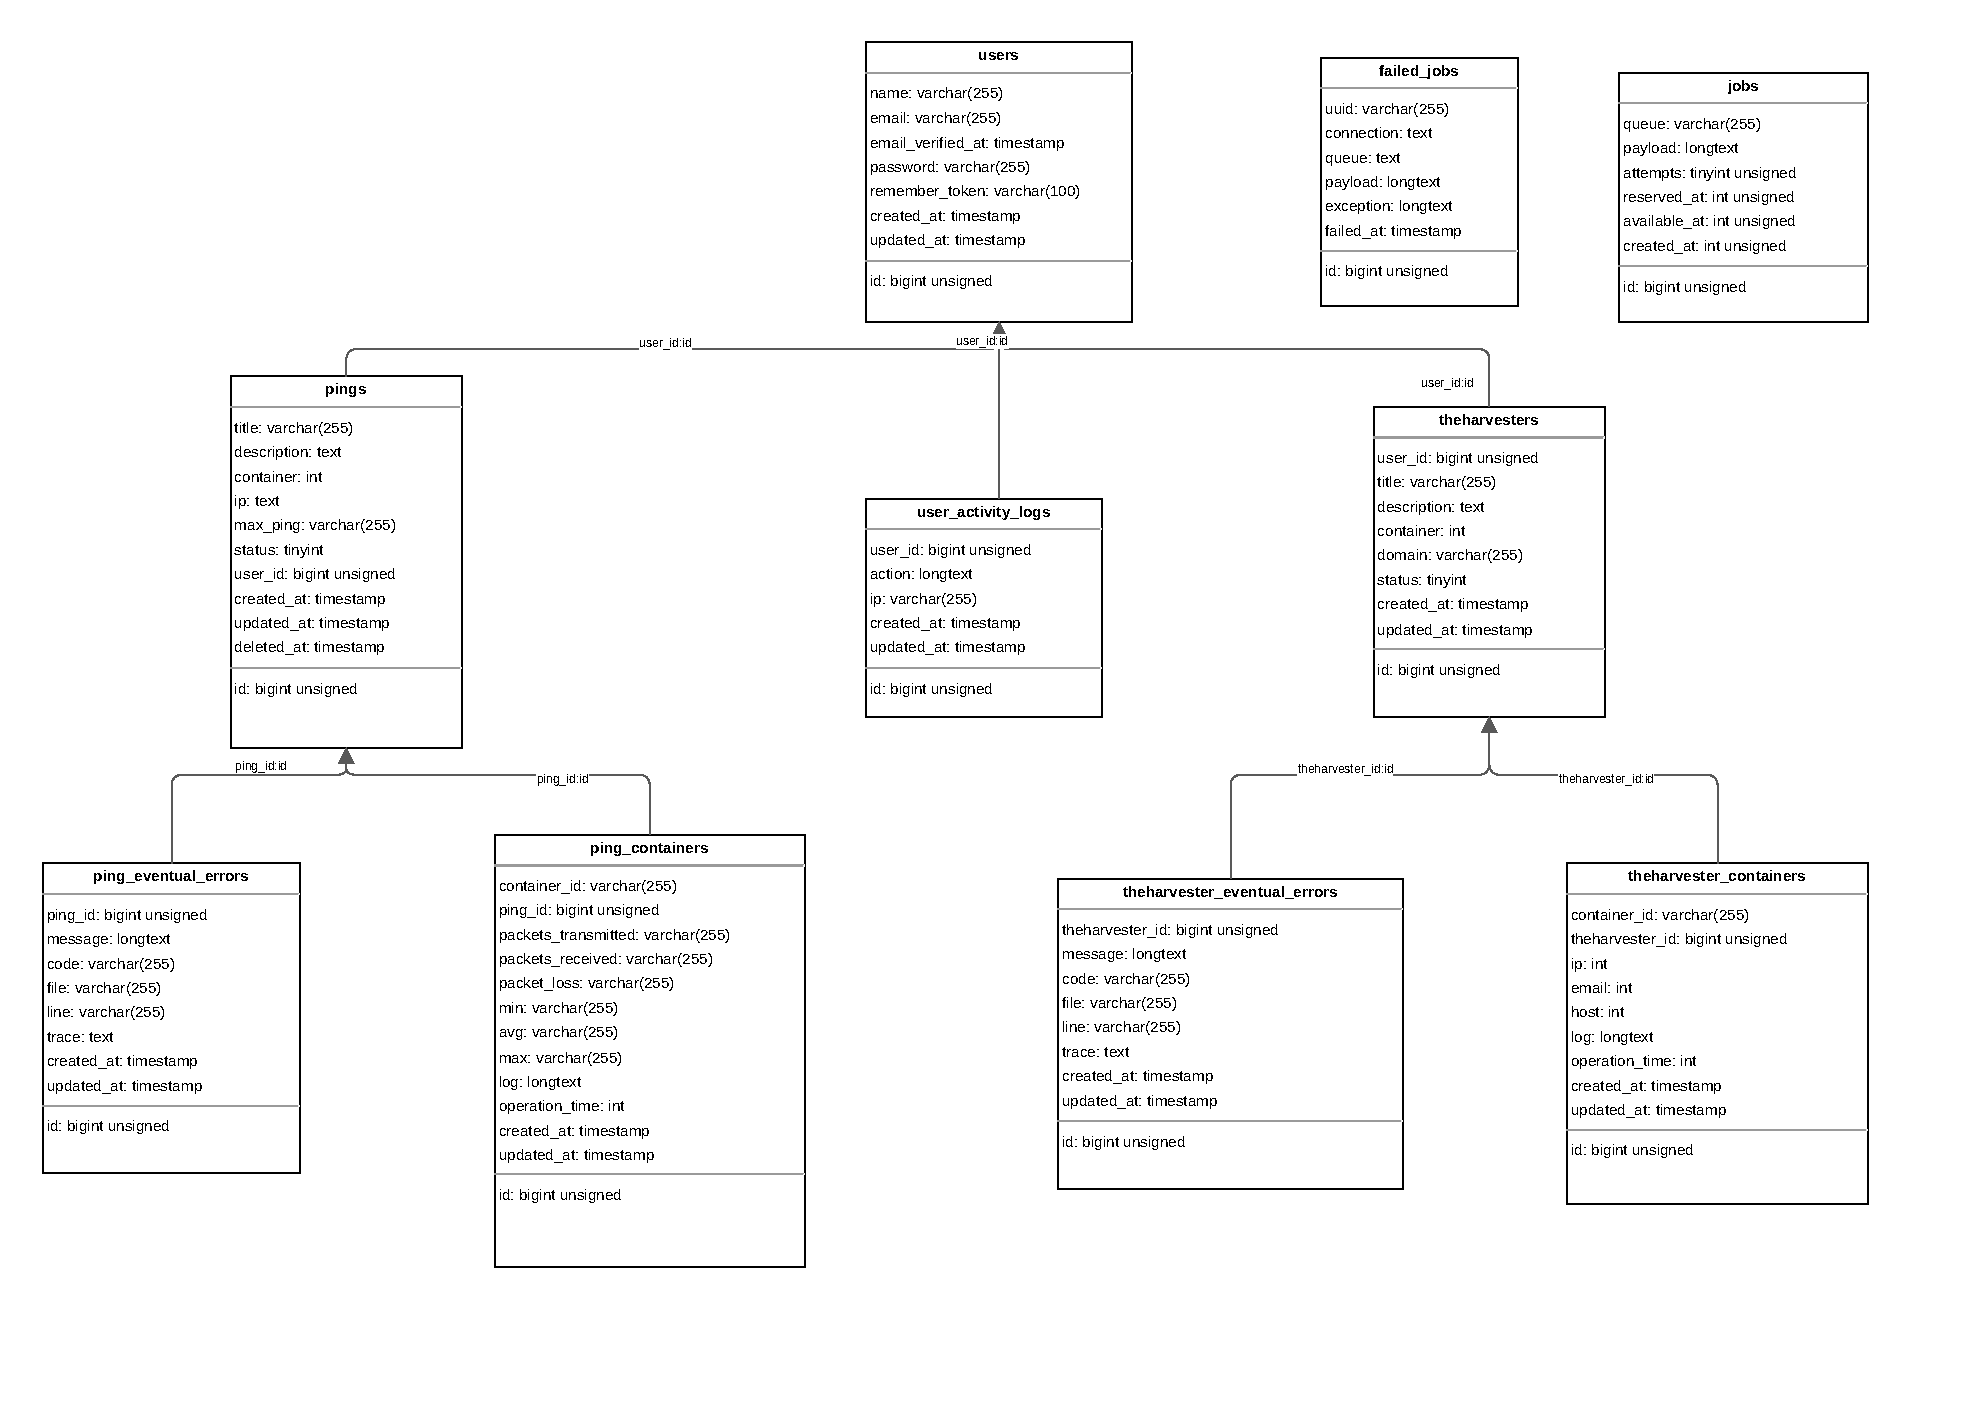
\includegraphics[width=\linewidth]{images/exported_from_idea.drawio.pdf}
  \caption{Veritabanı şeması}
  \label{fig:veritabani_diyagrami}
  \end{figure}
\subsection{Konteyner ile İlgili Temel Bilgiler}
Konteyner, bir uygulamanın çalışması için gereken tüm bağımlılıkları ve bileşenleri bir araya getiren ve bu bileşenlerin izole edilmiş bir ortamda çalışmasını sağlayan bir yazılım paketleme ve dağıtım teknolojisidir. Konteynerler, bir uygulamanın tüm çalışma zamanı bağımlılıklarını içeren taşınabilir bir ortam sunar ve böylece uygulamaların farklı platformlarda tutarlı bir şekilde çalışmasını sağlar \cite{domenici_bravo}.

Konteynerlerin avantajları şunlardır:
\begin{itemize}
  \item Taşınabilirlik: Konteynerler, uygulamaların bir ortamdan diğerine sorunsuz bir şekilde taşınmasını sağlar. Konteynerlerin bağımsız bir şekilde çalışabilmesi, farklı işletim sistemleri, bulut platformları veya dağıtım ortamları arasında sorun yaşamadan hareket etmelerini sağlar.
  \item İzolasyon: Konteynerler, uygulamaların birbirlerinden ve ana işletim sisteminden izole bir şekilde çalışmasını sağlar. Her konteyner, kendi dosya sistemine, ağ bağlantılarına ve kaynaklara sahiptir. Bu, uygulamaların birbirlerinin kaynaklarını etkilemeden güvenli bir şekilde çalışmasını sağlar.
  \item Hızlı Dağıtım: Konteynerler, hızlı ve tutarlı bir şekilde dağıtılabilir. Konteyner imajları, uygulamaların ve bağımlılıklarının bir araya getirildiği taşınabilir bir formattır. Bu imajlar hızlı bir şekilde oluşturulabilir, paylaşılabilir ve dağıtılabilir, böylece uygulamaların hızlı bir şekilde çalıştırılması ve güncellenmesi mümkün olur.
  \item Ölçeklenebilirlik: Konteynerler, uygulamaların kolayca ölçeklendirilmesini sağlar. Konteyner tabanlı bir uygulamanın birden fazla kopyası aynı anda çalıştırılabilir ve bir yük dengeleyici kullanılarak trafiğin bu kopyalar arasında dengeli bir şekilde dağıtılması sağlanabilir. Bu, yüksek talepler altında uygulamaların performansını artırır.
\end{itemize}

Konteynerlerin dezavantajları şunlardır:
\begin{itemize}
  \item Karmaşıklık: Konteyner teknolojileri, bazı kullanıcılar için karmaşık olabilir. Konteynerlerin oluşturulması, yönetimi ve yapılandırılması konusunda ek bilgi ve beceri gerektirebilir. Bu nedenle, konteyner teknolojilerini kullanmak isteyen kullanıcıların bu teknolojilere aşina olmaları ve gerektiğinde destek almaları önemlidir.
  \item Bellek ve İşlemci Kullanımı: Konteynerlerin izolasyonu sağlamak için ek sistem kaynaklarına ihtiyaçları olabilir. Konteynerler, her biri kendi işletim sistemleri gibi davranırken, her bir konteynerin bellek ve işlemci kullanımı ek yük getirebilir. Bu, sistem kaynaklarının daha dikkatli bir şekilde yönetilmesini gerektirebilir.
  \item Veri Yönetimi: Konteynerler, genellikle veri yönetimi konusunda bazı zorluklar sunabilir. Konteynerlerin geçici doğası ve izole edilmiş dosya sistemleri, verilerin nasıl depolanacağı, paylaşılacağı ve korunacağı konusunda bazı ek adımlar gerektirebilir. Bu, uygulama geliştiricilerinin veri yönetimi stratejilerini dikkate almalarını gerektirir.
\end{itemize}

Konteyner teknolojileri, uygulamaları hızlı bir şekilde dağıtmak, taşımak ve ölçeklendirmek için güçlü bir araçtır. Ancak, her çalışmanin ihtiyaçlarına ve altyapısına bağlı olarak avantajları ve dezavantajları dikkate almak önemlidir.

Çalışmanın ne olduğunu nasıl çalıştığı Bölüm \ref{sec:study}'te detaylıca anlatılmıştır.